\section{Ejercicio 3}\label{sec:ej3}

Evaluamos en esta sección el frente de Pareto de soluciones obtenido.
Consideramos primero la forma de las soluciones obtenidas, a grandes rasgos. En
la figura \ref{fig:3-pareto-num-coms} vemos el frente de Pareto obtenido,
junto con el número de comunidades en cada solución. Como esperábamos, cuanto
más se prioriza la densidad interna, en más comunidades se dividen los nodos, y
al revés con el \emph{average out-degree fraction}.

\begin{figure}[!htb]
  \centering
  \begin{subfigure}{.48\textwidth}
    \centering
    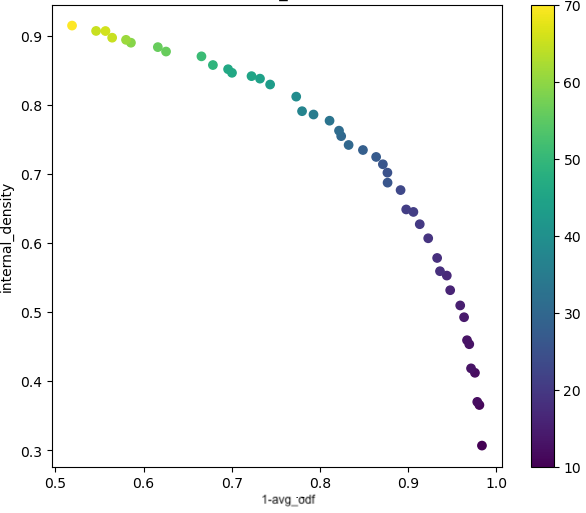
\includegraphics[width=\linewidth]{img/3_num_communities_pareto_1}
    \caption{Gráfico de los valores de \emph{fitness} de las soluciones del
    frente de Pareto obtenido. El eje $x$ representa el \(1-AVG\_ODF\), y el
    eje \(y\) la densidad interna media. El color representa el número de
    comunidades producidas.}
    \label{fig:3-pareto-num-coms-1}
  \end{subfigure}%
  \hfill
  \begin{subfigure}{.48\textwidth}
    \centering
    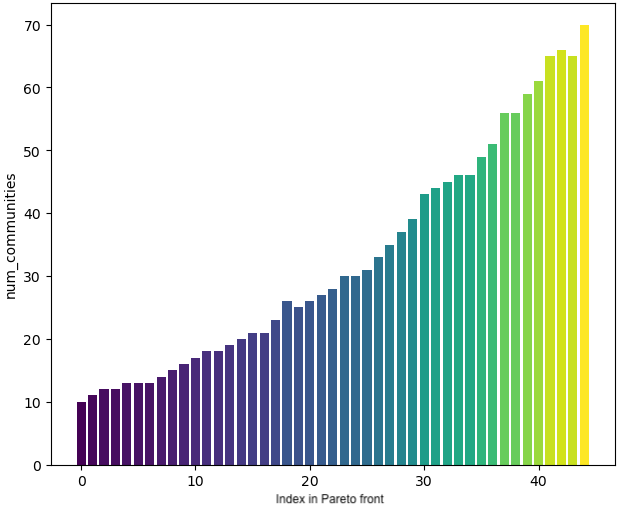
\includegraphics[width=\linewidth]{img/3_num_communities_pareto_2}
    \caption{Gráfico de barras del número de comunidades producidas. Las
      soluciones del frente de Pareto están ordenadas de menor \emph{average
      out-degree fraction} (izquierda) a mayor densidad interna (derecha). El
      eje \(y\) y el color representan la el valor de la información mutua
      respecto al \emph{ground truth}.}
  \label{fig:3-pareto-num-coms-2}
  \end{subfigure}
  \caption{Comparación del número de comunidades de las soluciones del frente
  de Pareto.}
  \label{fig:3-pareto-num-coms}
\end{figure}

Respecto a la información mutua con el \emph{ground truth}, vemos en la figura
\ref{fig:3-pareto-nmi} la comparación de dicha métrica entre las soluciones
del frente de Pareto. Es fácil ver que en general funciona mejor priorizar
bastante el \emph{average out-degree fraction}. Cogiendo la mejor solución
respecto a la información mutua, vemos en las figuras \ref{fig:3-circular-comp} y
\ref{fig:3-bipartite} la comparación de las comunidades obtenidas con las del
\emph{ground truth}. Observamos una solución ligeramente peor que la obtenida
\emph{tuneando} el parámetro de resolución en el algoritmo de Louvain, tanto
por el valor de la información mutua (\(0.6788 \leq 0.7\)) como gráficamente.

\begin{figure}[!htb]
  \centering
  \begin{subfigure}{.48\textwidth}
    \centering
    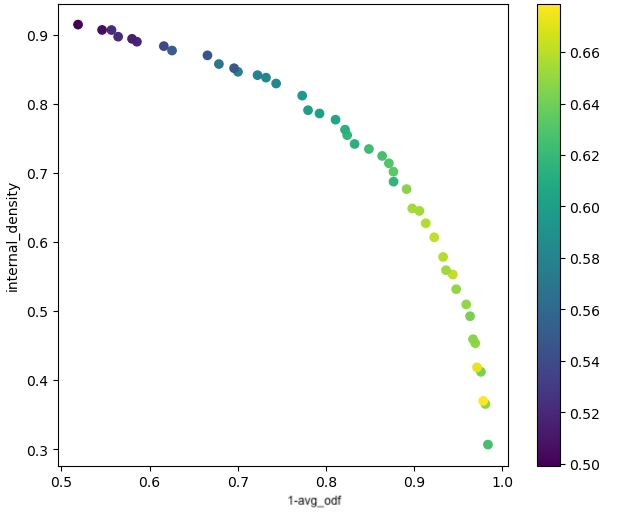
\includegraphics[width=\linewidth]{img/3_nmi_pareto_1}
    \caption{Gráfico de los valores de \emph{fitness} de las soluciones del
    frente de Pareto obtenido. El eje $x$ representa el \(1-AVG\_ODF\), y el
    eje \(y\) la densidad interna media. El color representa el valor de la
    información mutua respecto al \emph{ground truth}.}
    \label{fig:3-pareto-nmi-1}
  \end{subfigure}%
  \hfill
  \begin{subfigure}{.48\textwidth}
    \centering
    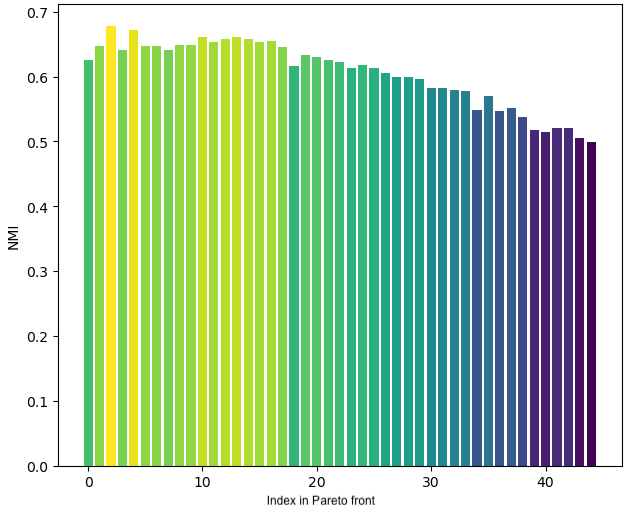
\includegraphics[width=\linewidth]{img/3_nmi_pareto_2}
    \caption{Gráfico de barras de la información mutua respecto al \emph{ground
      truth}. Las soluciones del frente de Pareto están ordenadas de menor
      \emph{average out-degree fraction} (izquierda) a mayor densidad interna
      (derecha). El eje \(y\) y el color representan la el valor de la
      información mutua respecto al \emph{ground truth}.}
  \label{fig:3-pareto-nmi-2}
  \end{subfigure}
  \caption{Comparación de la información mutua respecto al \emph{ground truth}
  de las soluciones del frente de Pareto.}
  \label{fig:3-pareto-nmi}
\end{figure}

\begin{figure}[!htb]
  \centering
  \begin{subfigure}{.4\textwidth}
    \centering
    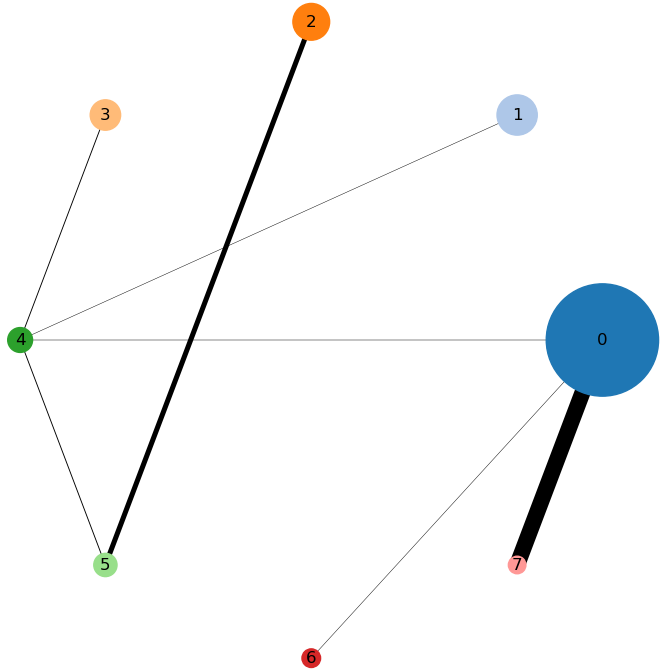
\includegraphics[width=.9\linewidth]{img/1_circular_comp_1}
    \caption{Gráfico circular de las comunidades \emph{ground truth}. }
    \label{fig:3-circular-comp-1}
  \end{subfigure}%
  \hfill
  \begin{subfigure}{.4\textwidth}
    \centering
    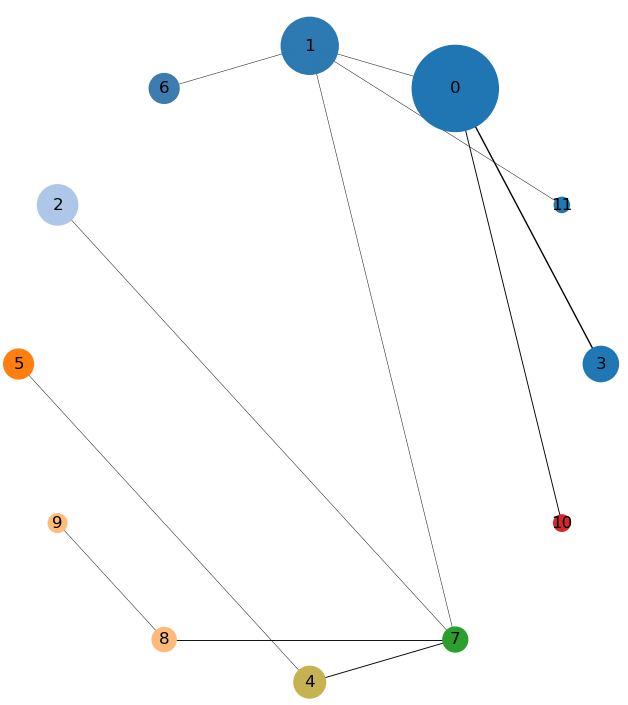
\includegraphics[width=.9\linewidth]{img/3_best_sol_circular_comp_2}
    \caption{Gráfico circular de las comunidades generadas por la mejor
      solución del algoritmo \emph{NSGA-II}. }
    \label{fig:3-circular-comp-2}
  \end{subfigure}
  \caption{Comparación de comunidades mediante un grafo bipartito. A la
    izquierda vemos las comunidades \emph{ground truth}, y a la derecha la
    mejor solución según la información mutua generada por \emph{NSGA-II}. Los
    colores de las comunidades en el gráfico de la derecha son una media de los
    del gráfico de la izquierda, en función del tamaño de la intersección con la
    comunidad correspondiente.}
  \label{fig:3-circular-comp}
\end{figure}

\begin{figure}[!htb]
  \centering
  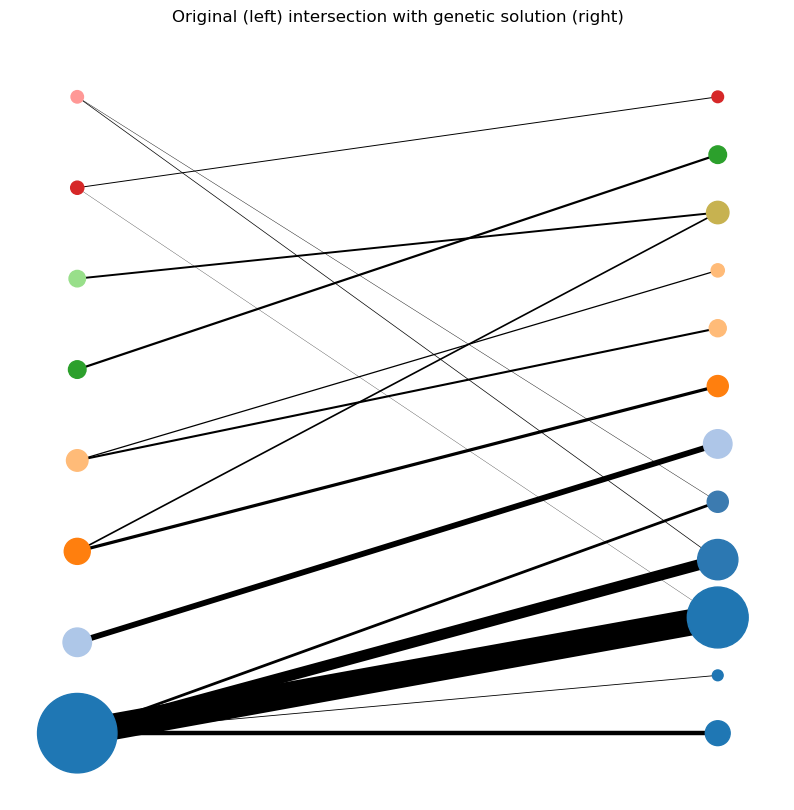
\includegraphics[width=.7\linewidth]{img/3_best_sol_bipartite_comp}
  \caption{Comparación de comunidades mediante un grafo bipartito. A la
    izquierda vemos las comunidades \emph{ground truth}, y a la derecha la
    mejor solución según la información mutua generada por \emph{NSGA-II}. Los
    colores de las comunidades en el gráfico de la derecha son una media de los
    del gráfico de la izquierda, en función del tamaño de la intersección con
    la comunidad correspondiente. Los tamaños de las aristas son tan gruesos
    como el número de nodos en común de las comunidades que conectan.}
  \label{fig:3-bipartite}
\end{figure}
